%%%%%%%%%%%%%%%%%%%%%%%%%%%%%%%%%%%%%%%%%
% Beamer Presentation
% LaTeX Template
% Version 1.0 (10/11/12)
%
% This template has been downloaded from:
% http://www.LaTeXTemplates.com
%
% License:
% CC BY-NC-SA 3.0 (http://creativecommons.org/licenses/by-nc-sa/3.0/)
%
% Modified by Nicholas J. Gotelli
% 9 January 2021
%%%%%%%%%%%%%%%%%%%%%%%%%%%%%%%%%%%%%%%
\documentclass[12pt]{beamer}\usepackage[]{graphicx}\usepackage[]{color}
% maxwidth is the original width if it is less than linewidth
% otherwise use linewidth (to make sure the graphics do not exceed the margin)
\makeatletter
\def\maxwidth{ %
  \ifdim\Gin@nat@width>\linewidth
    \linewidth
  \else
    \Gin@nat@width
  \fi
}
\makeatother

\definecolor{fgcolor}{rgb}{0.345, 0.345, 0.345}
\newcommand{\hlnum}[1]{\textcolor[rgb]{0.686,0.059,0.569}{#1}}%
\newcommand{\hlstr}[1]{\textcolor[rgb]{0.192,0.494,0.8}{#1}}%
\newcommand{\hlcom}[1]{\textcolor[rgb]{0.678,0.584,0.686}{\textit{#1}}}%
\newcommand{\hlopt}[1]{\textcolor[rgb]{0,0,0}{#1}}%
\newcommand{\hlstd}[1]{\textcolor[rgb]{0.345,0.345,0.345}{#1}}%
\newcommand{\hlkwa}[1]{\textcolor[rgb]{0.161,0.373,0.58}{\textbf{#1}}}%
\newcommand{\hlkwb}[1]{\textcolor[rgb]{0.69,0.353,0.396}{#1}}%
\newcommand{\hlkwc}[1]{\textcolor[rgb]{0.333,0.667,0.333}{#1}}%
\newcommand{\hlkwd}[1]{\textcolor[rgb]{0.737,0.353,0.396}{\textbf{#1}}}%
\let\hlipl\hlkwb

\usepackage{framed}
\makeatletter
\newenvironment{kframe}{%
 \def\at@end@of@kframe{}%
 \ifinner\ifhmode%
  \def\at@end@of@kframe{\end{minipage}}%
  \begin{minipage}{\columnwidth}%
 \fi\fi%
 \def\FrameCommand##1{\hskip\@totalleftmargin \hskip-\fboxsep
 \colorbox{shadecolor}{##1}\hskip-\fboxsep
     % There is no \\@totalrightmargin, so:
     \hskip-\linewidth \hskip-\@totalleftmargin \hskip\columnwidth}%
 \MakeFramed {\advance\hsize-\width
   \@totalleftmargin\z@ \linewidth\hsize
   \@setminipage}}%
 {\par\unskip\endMakeFramed%
 \at@end@of@kframe}
\makeatother

\definecolor{shadecolor}{rgb}{.97, .97, .97}
\definecolor{messagecolor}{rgb}{0, 0, 0}
\definecolor{warningcolor}{rgb}{1, 0, 1}
\definecolor{errorcolor}{rgb}{1, 0, 0}
\newenvironment{knitrout}{}{} % an empty environment to be redefined in TeX

\usepackage{alltt}
% only 10,11, or 12 pt fonts
% PACKAGES-----------------------------------
\usepackage{graphicx} % Allows including images
\usepackage{booktabs} % Allows the use of \toprule, \midrule and \bottomrule in tables

% NOTE:
%------
% This is what I added to resolve the following error:
% !pdfTeX error: pdflatex.exe (file mathkerncmssi12): Font mathkerncmssi12 at 600 not found
\pdfmapfile{+sansmathaccent.map}

% THEMES AND COLORS-------------------------
\mode<presentation> {
\usefonttheme{default}
% FONTTHEMES: default, structurebold, structuresmallcapsserif, structureitalicserif, serif, professionalfonts


\usetheme{Berlin}
% THEMES: default, AnnArbor, Antibes, Bergen, Berkeley, Berlin, Boadilla, boxes, CambridgeUS, Copenhagen, Darmstadt, Dresden, Frankfurt, Goettingen, Hannover, Ilmenau, JuanLesPins, Luebeck, Madrid, Malmoe, Marburg, Montpellier, PaloAlto, Pittsburgh, Rochester, Singapore, Szeged, Warsaw

\usecolortheme{dolphin}
%COLORTHEMES: default, albatross, beaver, beetle, crane, dolphin, dove, fly, lily, orchid, rose, seagull, seahorse, sidebartab, structure, whale, wolverine 

% DISPLAY OPTIONS--------------------------
%\setbeamertemplate{footline} % To remove the footer line in all slides, uncomment this line

%\setbeamertemplate{footline}[page number] % To replace the footer line in all slides with a simple slide count, uncomment this line

%\setbeamertemplate{navigation symbols}{} % To remove the navigation symbols from the bottom of all slides, uncomment this line
}
% -----------------------------------------

% TITLE PAGE DATA--------------------------
\title[Short title]{Melica Flowering Evolution} % The short title appears at the bottom of every slide, the full title is only on the title page

\author{Masoumeh Khodaverdi} % Your name

\institute[UVM] % Your institution as it will appear on the bottom of every slide, may be shorthand to save space
{
University of Vermont \\ % Your institution for the title page
Department of Plant Biology \\
Burlington, VT 05401 USA \\ 
\medskip
\textit{mkhodave@uvm.edu} % Your email address
}
\date{Febrarury 2021} % Date, can be changed to a custom date or \today
% -----------------------------------------

% BEGIN DOCUMENT---------------------------
\IfFileExists{upquote.sty}{\usepackage{upquote}}{}
\begin{document}

% OPTIONAL TITLE PAGE SLIDE----------------
\begin{frame}
\titlepage % Print the title page as the first slide
\end{frame}

% OPTIONAL TABLE OF CONTENTS SLIDE---------

\begin{frame}
\frametitle{Contents} % Table of contents slide, comment this block out to remove it
\tableofcontents % Throughout your presentation, if you choose to use \section{} and \subsection{} commands, these will automatically be printed on this slide as an overview of your presentation
\end{frame}

% OPTIONAL SECTION HEADERS-----------------
\section{My PhD} % Sections can be created in order to organize your presentation into discrete blocks; all sections and subsections are automatically printed in the table of contents as an overview of the talk

\subsection{My Lab} % A subsection can be created just before a set of slides with a common theme to further break down your presentation into chunks

% SLIDE (BULLET POINTS)--------------------
\begin{frame}
\frametitle{Lab Equipments}
\begin{itemize}
\item Here's a list of equipments we have in our lab:
\begin{itemize}
\item Pipette
\item PCR
\item ...
\end{itemize}
\end{itemize}
\end{frame}

\subsection{My Research}
% SLIDE (SEQUENTIAL BULLET POINTS)---------
\begin{frame}
\frametitle{Samples}
\begin{itemize}
\item<1-> I work on Melica Ciliata species
\item<2-> Here's a photo of it:

\vspace{.25cm}
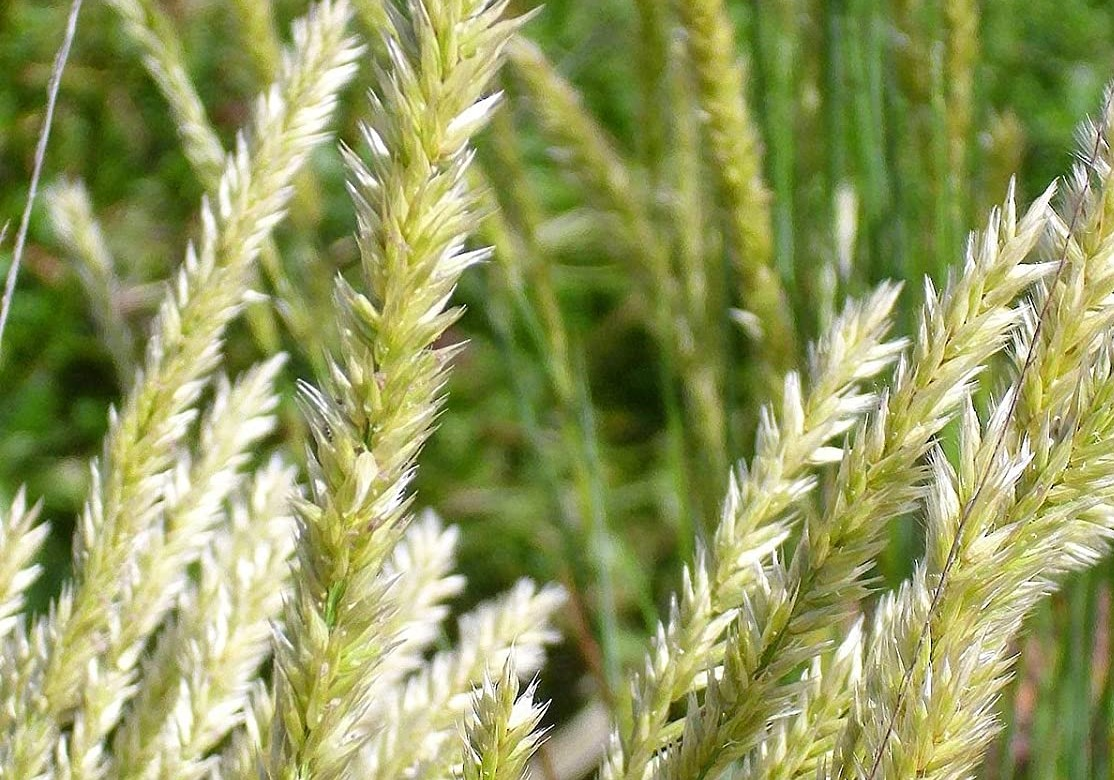
\includegraphics[width=0.5\columnwidth]{melica_ciliata.jpg}
\end{itemize}

\end{frame}



%------------------------------------------------
\section{My Life}
%------------------------------------------------
% SLIDE (PARAGRAPHS OF TEXT)---------------
\begin{frame}
\frametitle{What I Do Other than Research}
\begin{itemize}
  \item I like to travel.
  \item I enjoy cooking.
  \item I keep redecorating my place.
\end{itemize}
\end{frame}

\section{My Course}

% SLIDE (EMBEDDED R CODE)------------------
\begin{frame}[fragile]{Embedded R Code; \texttt{fragile} frame}
\begin{block}

\begin{knitrout}
\definecolor{shadecolor}{rgb}{0.969, 0.969, 0.969}\color{fgcolor}\begin{kframe}
\begin{alltt}
\hlcom{# show some output...}
\hlkwd{runif}\hlstd{(}\hlnum{10}\hlstd{)}
\end{alltt}
\begin{verbatim}
##  [1] 0.1734904943 0.8277370634 0.1636265144 0.1285929831 0.9582736911
##  [6] 0.1460577904 0.1161922347 0.2019316193 0.0009096595 0.2683320467
\end{verbatim}
\end{kframe}
\end{knitrout}

\end{block}
\end{frame}

% SLIDE (EMBEDDED R FIGURE)----------------
\begin{frame}[fragile]{Embedded R Figure; \texttt{fragile} frame}
%\begin{block}

\begin{knitrout}
\definecolor{shadecolor}{rgb}{0.969, 0.969, 0.969}\color{fgcolor}

{\centering 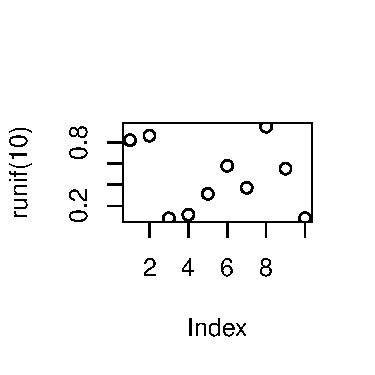
\includegraphics[width=\maxwidth]{figure/unnamed-chunk-2-1} 

}



\end{knitrout}

%\end{block}
\end{frame}

% SLIDE (MULTIPLE COLUMNS)-----------------
\begin{frame}
\frametitle{Multiple Columns}
\begin{columns}[c] % The "c" option specifies centered vertical alignment while the "t" option is used for top vertical alignment

\column{.45\textwidth} % Left column and width
\textbf{Heading}
\begin{enumerate}
\item Statement
\item Explanation
\item Example
\end{enumerate}

\column{.5\textwidth} % Right column and width
Lorem ipsum dolor sit amet, consectetur adipiscing elit. Integer lectus nisl, ultricies in feugiat rutrum, porttitor sit amet augue. Aliquam ut tortor mauris. Sed volutpat ante purus, quis accumsan dolor.

\end{columns}
\end{frame}


% SLIDE (THEOREM)----------------------------
\begin{frame}
\frametitle{Theorem}
\begin{theorem}[Mass--energy equivalence]
$E = mc^2$
\end{theorem}
\end{frame}

% SLIDE (VERBATIM)---------------------------
\begin{frame}[fragile] % Need to use the fragile option when verbatim is used in the slide
\frametitle{Verbatim}
\begin{example}[Theorem Slide Code]
\begin{verbatim}
\begin{frame}
\frametitle{Theorem}
\begin{theorem}[Mass--energy equivalence]
$E = mc^2$
\end{theorem}
\end{frame}\end{verbatim}
\end{example}
\end{frame}

% SLIDE (FINAL SLIDE)------------------------
\begin{frame}
\Huge{\centerline{Done for Now!}}
\end{frame}

%------------------------------------------------
\end{document}
